\documentclass[11pt,a4paper]{article}
\usepackage[utf8]{inputenc}
\usepackage[T1]{fontenc}
\usepackage{lmodern}
\usepackage[margin=2.5cm]{geometry}
\usepackage{amsmath,amssymb}
\usepackage{graphicx,booktabs,longtable,array,float,calc}
\usepackage{enumitem}
\usepackage{microtype}
\usepackage[hidelinks]{hyperref}
\usepackage{url}
\urlstyle{same}
\Urlmuskip=0mu plus 1mu
\emergencystretch=2em
\setlist{itemsep=1pt,topsep=3pt,parsep=0pt}
\setlength{\parskip}{4pt}
\setlength{\parindent}{0pt}
\providecommand{\tightlist}{\setlength{\itemsep}{1pt}\setlength{\parskip}{0pt}}
\DeclareUnicodeCharacter{2212}{\ensuremath{-}}
\DeclareUnicodeCharacter{0394}{\ensuremath{\Delta}}
\DeclareUnicodeCharacter{03C0}{\ensuremath{\pi}}
\DeclareUnicodeCharacter{03B3}{\ensuremath{\gamma}}
\DeclareUnicodeCharacter{03B1}{\ensuremath{\alpha}}
\DeclareUnicodeCharacter{03B5}{\ensuremath{\varepsilon}}
\DeclareUnicodeCharacter{03B2}{\ensuremath{\beta}}
\DeclareUnicodeCharacter{03BC}{\ensuremath{\mu}}
\DeclareUnicodeCharacter{2192}{\ensuremath{\rightarrow}}
\DeclareUnicodeCharacter{2265}{\ensuremath{\geq}}
\DeclareUnicodeCharacter{2264}{\ensuremath{\leq}}
\DeclareUnicodeCharacter{2248}{\ensuremath{\approx}}
\DeclareUnicodeCharacter{2082}{\ensuremath{_2}}
\renewcommand{\arraystretch}{1.15}
\setlength{\tabcolsep}{4pt}
\setkeys{Gin}{keepaspectratio}
\usepackage[font=small,labelfont=bf]{caption}

\title{A Few Bits Suffice:\\[2pt]\large Breaking and Auditing Tacit Collusion Between Learning Pricing Agents}
% TODO: replace with your name and affiliation before submitting
\author{manuaishika\\ \small Independent researcher}
\date{}

\begin{document}
\maketitle

\begin{abstract}
Pricing agents can learn to collude without communicating: in repeated markets, independent learners settle on high prices and punish rivals who undercut. A regulator or platform needs to know which restrictions break such collusion, and what evidence separates it from prices that are high by coincidence. We study both in the standard logit-demand pricing game of Calvano et al.~(2020). We train Q-learning agents in about 10,000 sessions, restricting what they can see of their rival's price, and compare them with control agents that reach high prices but cannot sustain collusion. We also ask a question that becomes central for AI agents: does looking \emph{inside} an agent, at what it intends to do, reveal collusion that watching what it does misses?

Five results:

\begin{enumerate}
\def\labelenumi{\arabic{enumi}.}
\tightlist
\item
  \textbf{A few bits suffice, if they are the right bits.} Telling agents only whether the rival's price is in the upper or lower half of the range (one bit) leaves collusion almost intact (collusion index 0.81 → 0.75), as does showing it relative to their own price as lower, equal or higher (1.6 bits, 0.73). A one-bit relative signal (``is the rival at least as high as me?'') cuts it to 0.50.
\item
  \textbf{Corrupting or delaying the signal works where banding does not.} Random noise (−53\%) and a one-period delay (−41\%) cut collusion. Delay removes no information; it works mainly because fewer agents learn to retaliate (86\% → 41\%), not because punishment would arrive too late for a perfect trigger strategy.
\item
  \textbf{Collusion is a private convention.} Agents from different sessions cannot collude with each other (0.20), but a new entrant re-learns collusion within one training run (0.74).
\item
  \textbf{Standard evidence fails at equal price levels.} In 280 matched pairs, price level is at chance (AUC 0.48) and parallel pricing points the wrong way (0.02). Testing whether a firm \emph{reacts} to its rival's price changes detects collusion well (0.91).
\item
  \textbf{Behaviour understates intent.} Colluders who see their rival through noise \emph{intend} to retaliate about twice as hard as they actually do in the market (−0.27 vs.~−0.14). Reading each agent's learned strategy detects collusion better (AUC 0.89) than any behavioural test (≤ 0.78).
\end{enumerate}

These conclusions hold across three alternative learning-parameter settings and do not depend on training length. The takeaway is that defenders should corrupt or delay coordination signals rather than coarsen them, and auditors should test reactions, not price levels or parallelism, and should ask for access to agents' internals where they can. We release a tested LLM-agent version of the same experiments in which the ``internals'' are the agents' written reasoning, together with pre-registered predictions.

\end{abstract}

\hypertarget{introduction}{%
\section{Introduction}\label{introduction}}

Firms increasingly delegate pricing to algorithms, and increasingly to AI agents. Independent reinforcement-learning (RL) agents learn supracompetitive prices sustained by punishment, without being told to collude (Calvano et al., 2020; Klein, 2021). LLM agents do the same (Fish et al., 2024). This is a clean instance of a multi-agent failure: each agent faithfully serves its principal, and together they harm consumers (Hammond et al., 2025). It is also hard to police, because there is no agreement to prosecute (Harrington, 2018).

We ask four questions:

\begin{itemize}
\tightlist
\item
  \textbf{RQ1 (defender).} Which single restriction on what agents observe removes the most collusion, and at what cost?
\item
  \textbf{RQ2 (robustness of collusion).} Does collusion survive replacing one of the agents?
\item
  \textbf{RQ3 (auditor).} What \emph{behavioural} evidence separates collusion from coincidence? Agents can price high for benign reasons such as imperfect learning (Abada \& Lambin, 2023), and the ``plus factors'' used in antitrust, notably parallel pricing, may not separate the two cases.
\item
  \textbf{RQ4 (what agents intend vs.~what they do).} Does looking inside an agent reveal collusion that its behaviour hides? For Q-learners, ``inside'' is the learned strategy. For LLM agents it would be their written reasoning. We answer RQ4 for Q-learners and leave the LLM version as an open, pre-registered question.
\end{itemize}

We answer these in a setting where ground truth is known by construction: we control whether an agent \emph{can} condition on its rival and \emph{values} the future, independently of the prices it ends up charging.

Our contributions:

\begin{enumerate}
\def\labelenumi{\arabic{enumi}.}
\tightlist
\item
  \textbf{A cost map of five interventions on the price signal.} Collusion survives coarsening to one or two well-chosen bits, but random corruption and delay break it. We measure costs in bits withheld and in welfare, and test why delay works: it mainly stops agents from learning to retaliate.
\item
  \textbf{Evidence that learned collusion is a pair-specific convention.} Cross-play removes it; entry restores it.
\item
  \textbf{A labelled benchmark for telling collusion from coincidence.} At matched price levels, high prices and parallel pricing fail as evidence, while reaction-based tests succeed.
\item
  \textbf{A comparison of reading an agent's mind with watching its hands.} On the same sessions, an auditor that reads agents' learned strategies outperforms every behavioural test overall, and shows that observation noise hides about half of agents' intended retaliation.
\item
  \textbf{An open, tested LLM-agent extension.} It reproduces the same interventions and probes, adds an LLM judge of agents' private notes (the ``say'' counterpart of reading the strategy), and comes with pre-registered predictions (Appendix B).
\end{enumerate}

\hypertarget{related-work}{%
\section{Related Work}\label{related-work}}

\textbf{Algorithmic collusion.} Calvano et al.~(2020) show that Q-learners in a repeated logit Bertrand game reach near-monopoly prices enforced by punishment, which they verify with an impulse-response test. We reuse that test as an auditor's probe. Klein (2021) finds the same under sequential pricing. Asker, Fershtman and Pakes (2022) show that outcomes depend on algorithm design. Fish et al.~(2024) find that LLM agents reach supracompetitive prices in the same environment.

\textbf{Remedies.} Johnson, Rhodes and Wildenbeest (2023) design platform rules that discipline pricing algorithms by steering demand. Abada and Lambin (2023) attribute seemingly collusive outcomes to imperfect exploration, which motivates our coincidence controls. We instead compare interventions on the \emph{information channel} on a common scale (bits withheld), and ask which \emph{kind} of information loss matters.

\textbf{Detection and collusion carriers.} Work on LLM collusion mostly audits explicit or steganographic messages (Motwani et al., 2024; \emph{Audit the Whisper}, 2025). We study the case where the carrier is the price signal itself and there is no text to inspect. We ask what behavioural evidence suffices. To our knowledge, no prior work evaluates behavioural detectors against labelled non-collusive agents at matched price levels. Concurrent work addresses neighbouring questions for LLM pricing agents: Lee and Park (2026) argue that monitoring chain-of-thought alone cannot be relied on to detect collusion, and Garra (2026) studies mitigations for emergent collusion. Our extension tests a related question, whether agents' written reasoning reveals intent that their prices hide, against a Q-learning counterpart, reading learned strategies, where the answer can be checked directly. We have read only the abstracts of these papers and do not compare results.

\hypertarget{methods}{%
\section{Methods}\label{methods}}

\begin{figure}
\centering
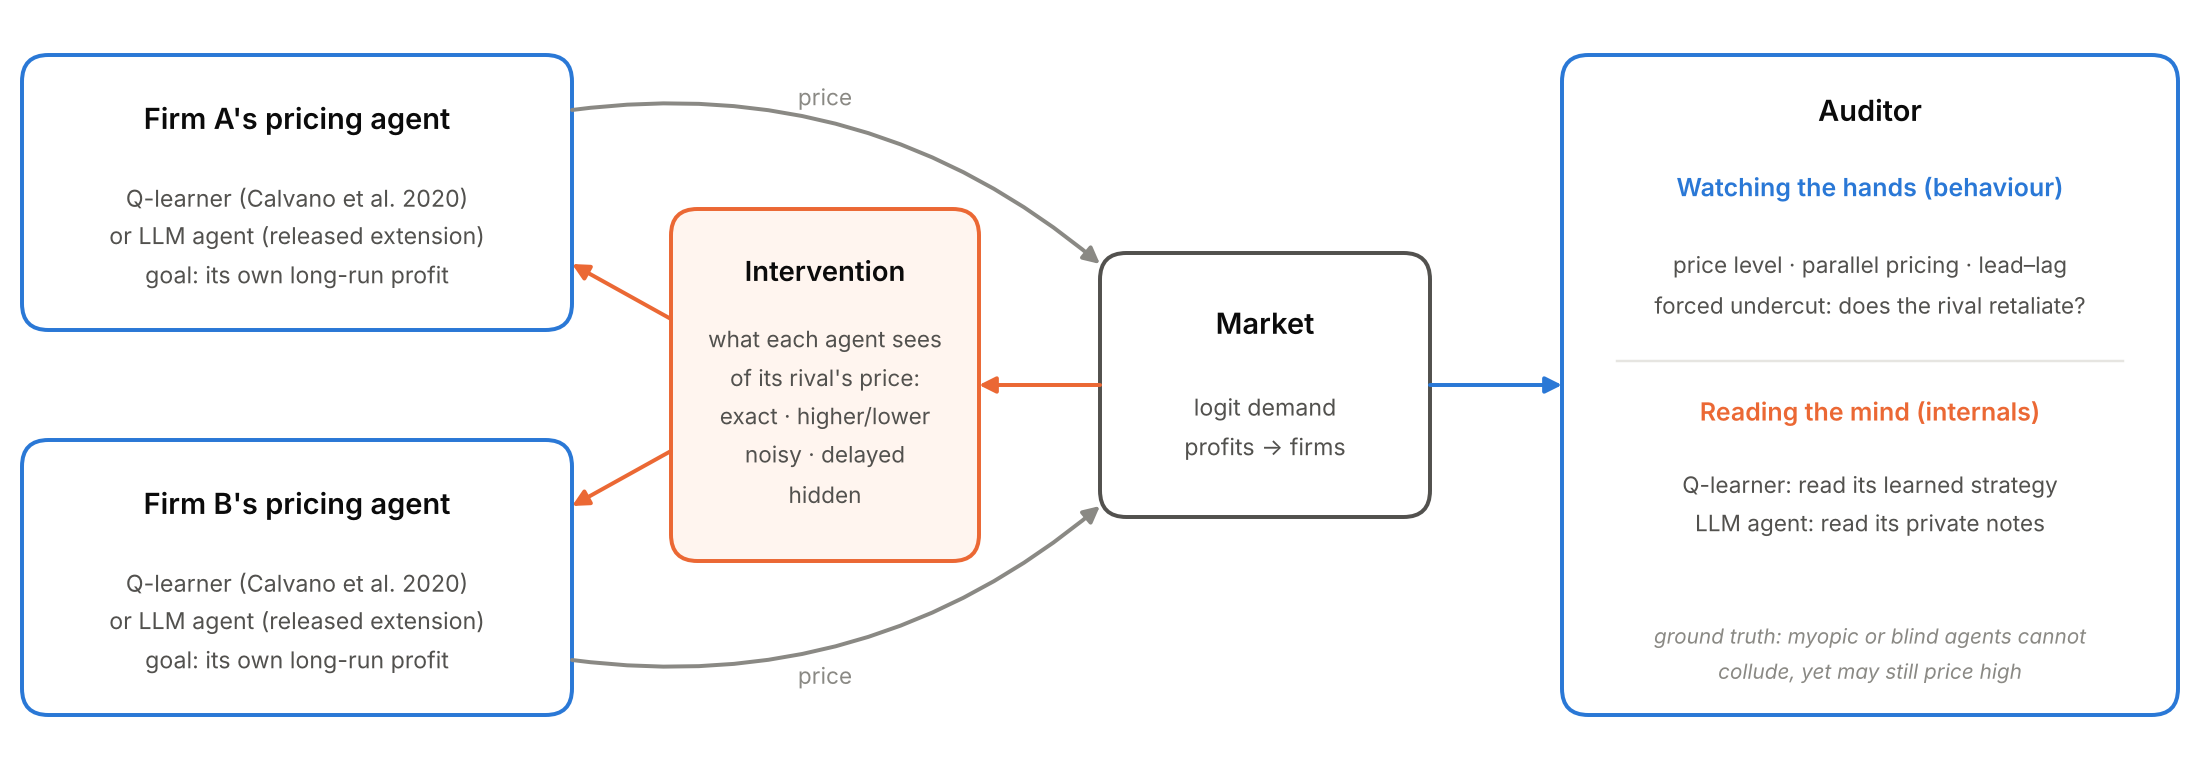
\includegraphics[width=0.95\textwidth,height=\textheight]{figures/setup.png}
\caption{Setup. Two Q-learning agents set prices in a logit-demand market. An intervention controls what each agent sees of its rival's price. An auditor either watches behaviour (prices, reactions, a forced one-period undercut) or reads the agents' internals (the learned strategy; for LLM agents, their private notes). Its task is to tell agents that can collude from agents that cannot but may still price high.}
\end{figure}

\textbf{Market.} We use the logit-demand Bertrand duopoly of Calvano et al.~(2020) with their parameters: quality 2, outside good 0, marginal cost 1, differentiation μ = 0.25. The static Nash price is \(p_{N}\) = 1.47 and the joint-monopoly price is \(p_{M}\) = 1.93, on a 15-point price grid. The \textbf{collusion index} is Δ = (π − \(π_{N}\))/(\(π_{M}\) − \(π_{N}\)), where 0 is competitive and 1 is monopoly.

\textbf{Agents.} Tabular Q-learning with one-period memory: the state is last period's observed prices. We use learning rate α = 0.15, discount γ = 0.95, exploration probability \(e^{-\beta t}\) with β = \(10^{-5}\), and Calvano et al.'s initialisation. Training stops once greedy policies are stable for \(10^{5}\) periods (at most 3×\(10^{6}\) periods), and outcomes are measured over the greedy play that follows. Each condition uses 100 seeds. Kernels are compiled with numba, and one session takes about 0.3 s on one CPU core.

\textbf{Interventions.} These act during training and deployment:

\begin{itemize}
\tightlist
\item
  \emph{noise}: each observed rival price is replaced by a random grid price with probability ε;
\item
  \emph{banding (absolute coarsening)}: the rival's price is observed only as one of k equal bands of the price grid (k = 2: upper or lower half; k = 1: nothing);
\item
  \emph{relative signals}: the rival's price is observed only relative to the agent's own last price, as lower / equal / higher (1.6 bits) or as ``at least as high as mine?'' (1 bit);
\item
  \emph{delay}: the rival's price is observed d periods late;
\item
  \emph{jitter}: each executed price is randomised with probability p;
\item
  \emph{blind}: the rival's price is never observed.
\end{itemize}

For noise and banding we report the information the agent retains about the rival's price, \(I(\text{true};\text{observed})\), under a uniform prior. At baseline this is \(\log_2 15\) = 3.9 bits.

\textbf{Swaps.} From 100 converged pairs we test three swaps:

\begin{itemize}
\tightlist
\item
  \emph{cross-play}: firm 0 of session s meets firm 1 of session s+1, with no further learning;
\item
  \emph{fresh entrant}: a new learner replaces firm 1 and both firms continue learning;
\item
  \emph{myopic entrant}: a learner with γ = 0 replaces firm 1.
\end{itemize}

\textbf{Auditing benchmark.} Positives are agents that can run a punishment scheme: γ = 0.95, with full or noisy (ε = 0.2) observation. Negatives are agents that cannot: myopic (γ = 0), short-horizon (γ = 0.5) and blind. Each condition has 1,000 seeds. We compare five detectors:

\begin{itemize}
\tightlist
\item
  D1, price level Δ;
\item
  D2, parallel pricing (correlation of the two firms' prices);
\item
  D3, lead--lag reaction, \(\mathrm{corr}(\Delta p_i(t), \Delta p_j(t{+}1))\), measured over 20,000 periods with 5\% random price noise;
\item
  D4, the active probe's punishment: the rival's next-period price response after firm 0 is forced to its one-shot best response, compared against an identical-seed replay without the deviation;
\item
  D5, the probe's payoff: the discounted gain from that deviation.
\end{itemize}

We report ROC AUC with 1,000-sample bootstrap 95\% CIs. The key comparison is \textbf{Δ-matched}: each myopic session with Δ \textgreater{} 0.1 is paired with a colluding session whose Δ differs by less than 0.02. This gives 280 pairs with a mean gap of 0.004, so a detector can succeed only by seeing the \emph{mechanism}, not the price level.

\textbf{Reading the strategy (white-box audit).} For each detection session we also read the agents' learned policies directly. Take the market's current state. For every lower price the rival could have charged instead, we look up what the responder's policy says it would charge next. \textbf{W} is the mean change from its on-path price, in units of \(p_{M}\) − \(p_{N}\); negative means it plans to retaliate. We read the policy at the true rival price, so observation noise does not blur it. This requires no market interaction. It is the Q-learning analogue of reading an LLM agent's notes. Sessions are deterministic given the seed, so this re-run reproduces the detection sessions exactly (identical Δ), and white-box and behavioural scores can be compared on the same agents.

\textbf{Robustness.} We re-run the five main levers (none, one absolute bit, 20\% noise, 1-period delay, blind) under three alternative settings, with 50 seeds each:

\begin{itemize}
\tightlist
\item
  Calvano et al.'s slower exploration, β = 4×\(10^{-6}\);
\item
  a lower learning rate, α = 0.1;
\item
  a higher learning rate, α = 0.25.
\end{itemize}

\textbf{Follow-up experiments.} Three further experiments answer specific questions raised by the main results.

\begin{itemize}
\tightlist
\item
  \emph{Relative signals:} 100 sessions for each relative signal above, compared with the absolute two-band signal.
\item
  \emph{Delay mechanism:} for delays of 0, 1, 2 and 4 periods (100 sessions each) we measure the rival's price response to a forced cut at every lag after it can first see the cut. We also measure the intended retaliation read from each agent's learned strategy, evaluated at the delayed state; a session \emph{learned to retaliate} if this is below −0.1(\(p_{M}\) − \(p_{N}\)). Finally we compute the highest symmetric price a grim-trigger scheme can sustain at γ = 0.95 when a deviation goes unpunished for 1 + delay periods.
\item
  \emph{Training length:} for jitter (p = 0.05, 0.1) and 20\% noise, 60 sessions at each of 1, 3, 6 and 12 million training periods.
\end{itemize}

\textbf{What didn't work, and a correction.} Our first matching used nearest neighbours without a caliper. Because the classes' Δ distributions overlap only partly, it left a 0.13 gap in Δ, and price level still looked diagnostic (AUC 0.89). Adding the caliper removed this artefact. Separately, an earlier version of this paper described the two-band signal as ``whether the rival's price is higher or lower than the agent's own''. It is absolute (upper versus lower half of the grid). Running the relative signals (Section 4.1) shows that the distinction matters.

\hypertarget{results}{%
\section{Results}\label{results}}

\textbf{Baseline.} Two Q-learners reach Δ = 0.81 (95\% CI 0.79--0.83), with 99\% of sessions above 0.5. A forced price cut is punished: the rival cuts its price by 0.41(\(p_{M}\) − \(p_{N}\)) the next period, and the deviation loses 1.34(\(π_{M}\) − \(π_{N}\)) in discounted profit. This reproduces Calvano et al.~(2020). Adding a third firm lowers Δ to 0.63.

\begin{figure}
\centering
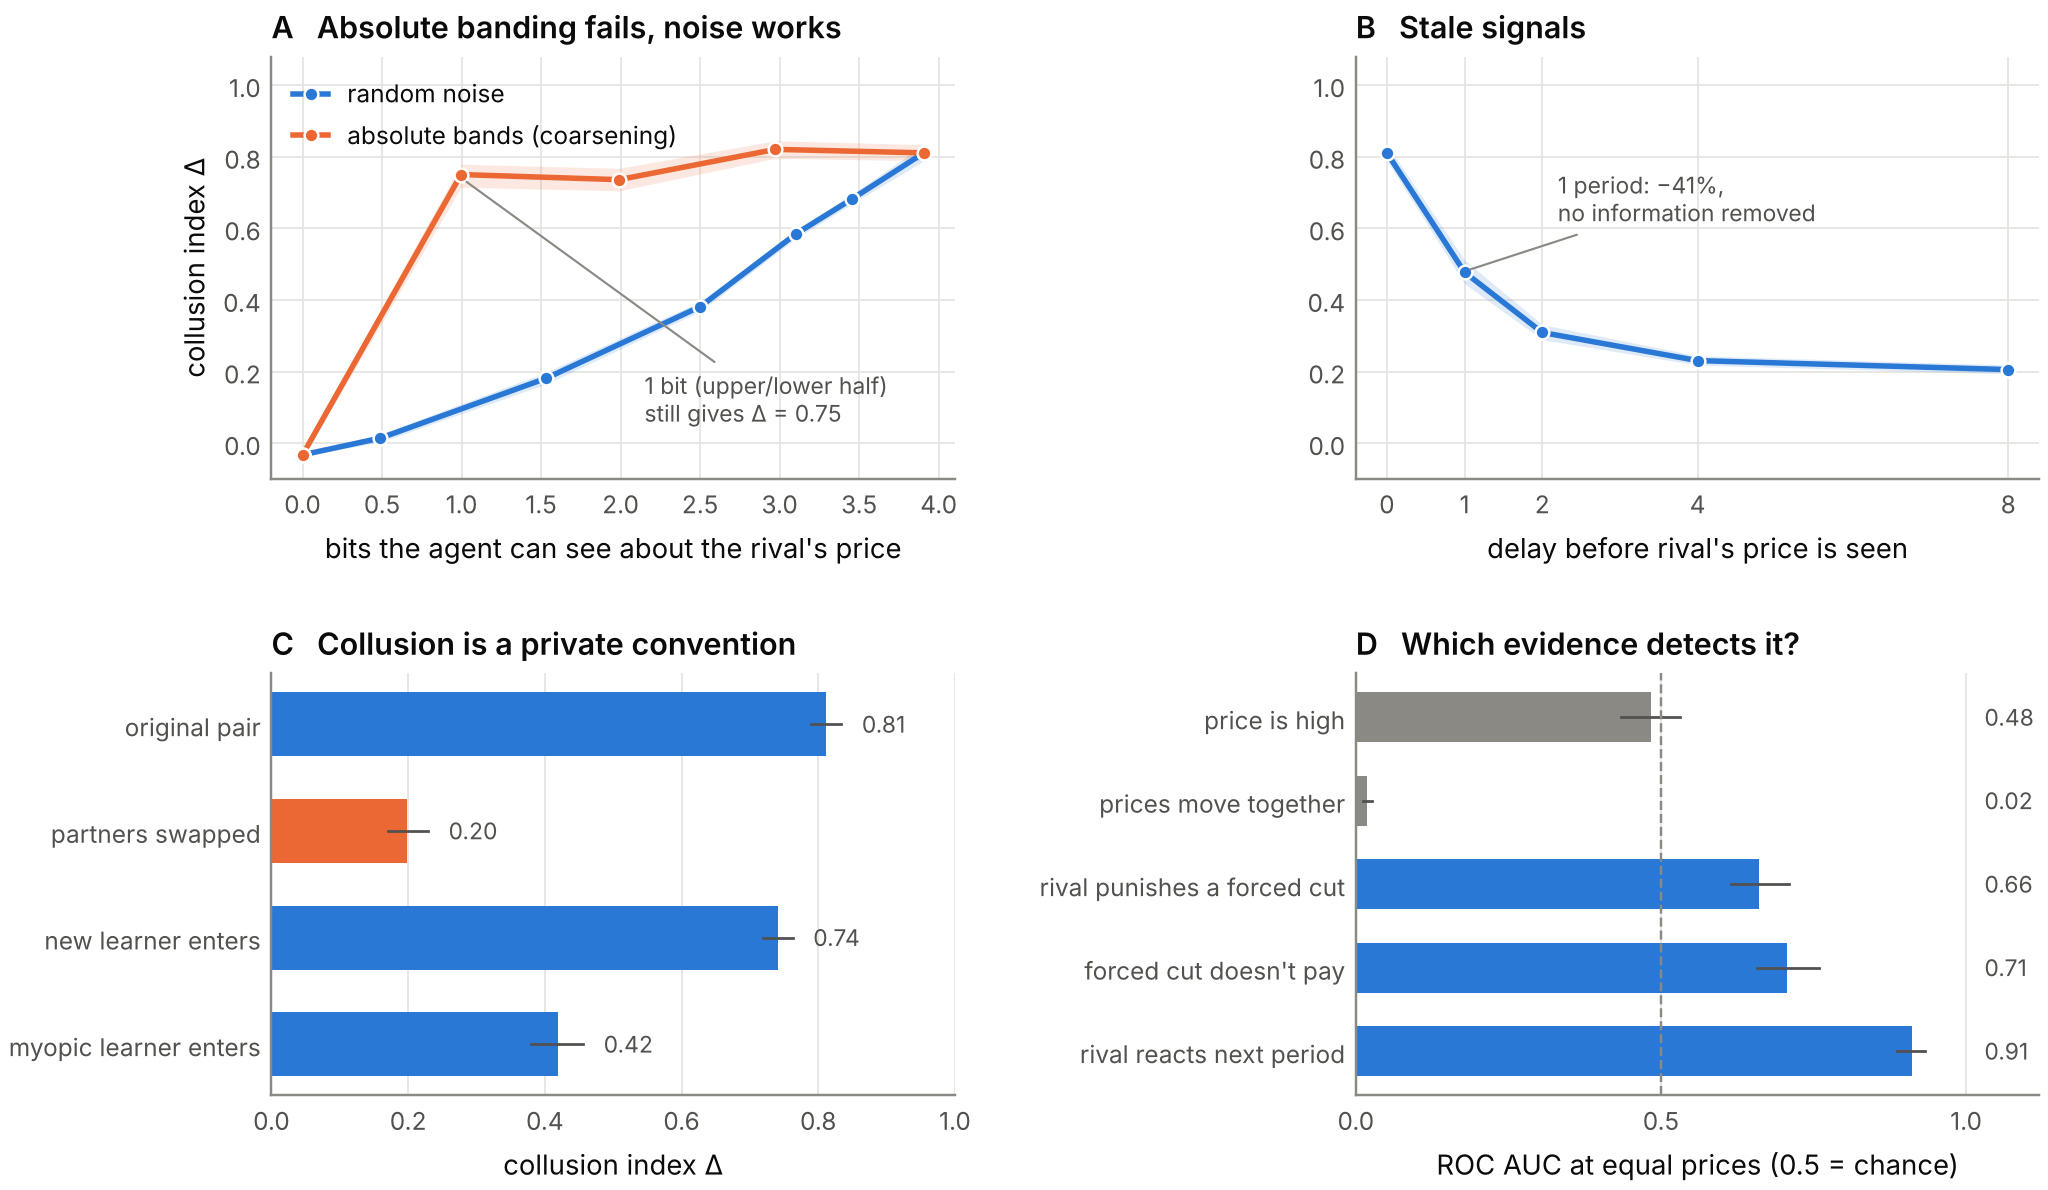
\includegraphics[width=0.82\textwidth,height=\textheight]{figures/rl_main.png}
\caption{Main results (100 sessions per point in A--C; 280 matched pairs in D; bands and bars are 95\% CIs).}
\end{figure}

\begin{itemize}
\tightlist
\item
  \emph{(A)} With the rival's price banded to one bit (upper or lower half), Δ stays at 0.75. Random noise withholding similar information cuts collusion far more.
\item
  \emph{(B)} A one-period delay cuts Δ by 41\% without removing any information.
\item
  \emph{(C)} Agents from different sessions fail to collude with each other, but a new learner re-learns collusion.
\item
  \emph{(D)} At equal price levels, ``price is high'' is at chance and ``prices move together'' is far below chance, while a lead--lag reaction test detects collusion.
\end{itemize}

\hypertarget{which-restriction-breaks-collusion}{%
\subsection{Which restriction breaks collusion?}\label{which-restriction-breaks-collusion}}

\begingroup\small\noindent

\emph{Table 1. Collusion under one dose of each intervention (100 sessions each). ``Bits removed'' is relative to 3.9 bits. ΔCS and ΔW are per-period changes in consumer surplus and total welfare relative to no intervention.}

\endgroup

\begingroup\small
\begin{longtable}[]{@{}lllll@{}}
\toprule\noalign{}
Intervention & Δ (95\% CI) & Bits removed & ΔCS & ΔW \\
\midrule\noalign{}
\endhead
\bottomrule\noalign{}
\endlastfoot
none & 0.81 (0.79--0.83) & 0 & -- & -- \\
1 absolute bit (upper/lower half) & 0.75 (0.71--0.78) & 2.9 & +0.03 & +0.02 \\
1-period delay & 0.48 (0.45--0.51) & 0 & +0.12 & +0.04 \\
5\% price jitter & 0.45 (0.41--0.49) & 0 & +0.12 & +0.04 \\
20\% noise & 0.38 (0.37--0.40) & 1.4 & +0.15 & +0.05 \\
2-period delay & 0.31 (0.29--0.33) & 0 & +0.18 & +0.06 \\
70\% noise & 0.01 (0.00--0.03) & 3.4 & +0.26 & +0.08 \\
blind & −0.03 (−0.04 to −0.02) & 3.9 & +0.27 & +0.08 \\
\end{longtable}
\endgroup

\begin{itemize}
\tightlist
\item
  \textbf{Banding does not help.} Even with only the upper or lower half of the price range visible (one bit), agents sustain Δ = 0.75 with full punishment (−0.43). A cut from collusive to competitive prices crosses the middle of the range, so one bit is enough to see it.
\item
  \textbf{Which one-bit signal matters (Figure 3A).} Showing the rival's price relative to the agent's own (``lower / equal / higher'', 1.6 bits) keeps Δ = 0.73 (0.71--0.75). Showing only ``at least as high as mine?'' (one bit) drops it to 0.50 (0.45--0.54), with weaker punishment (−0.19). The two-valued signal merges ``the rival matched me'' with ``the rival raised its price''. We read this as the signal needing to separate ``the rival is where I expect'' from ``the rival moved down'', but we have not tested that reading directly.
\item
  \textbf{Noise does help.} Withholding a similar amount of information as random noise cuts collusion far more: at 1.5 bits retained, Δ = 0.18 (Figure 2A). Random corruption makes the trigger fire against innocent rivals, and the scheme unravels.
\item
  \textbf{Delay helps without removing information.} A one-period delay cuts Δ by 41\%. Section 4.2 examines why.
\item
  \textbf{Nothing short of blindness fully works.} No moderate dose restores competition: delay and jitter level off near Δ ≈ 0.2. Only blindness, or noise at ε ≥ 0.7, reaches the Nash benchmark.
\item
  \textbf{Welfare improves throughout.} Every lever raised consumer surplus and total welfare.
\end{itemize}

\begin{figure}
\centering
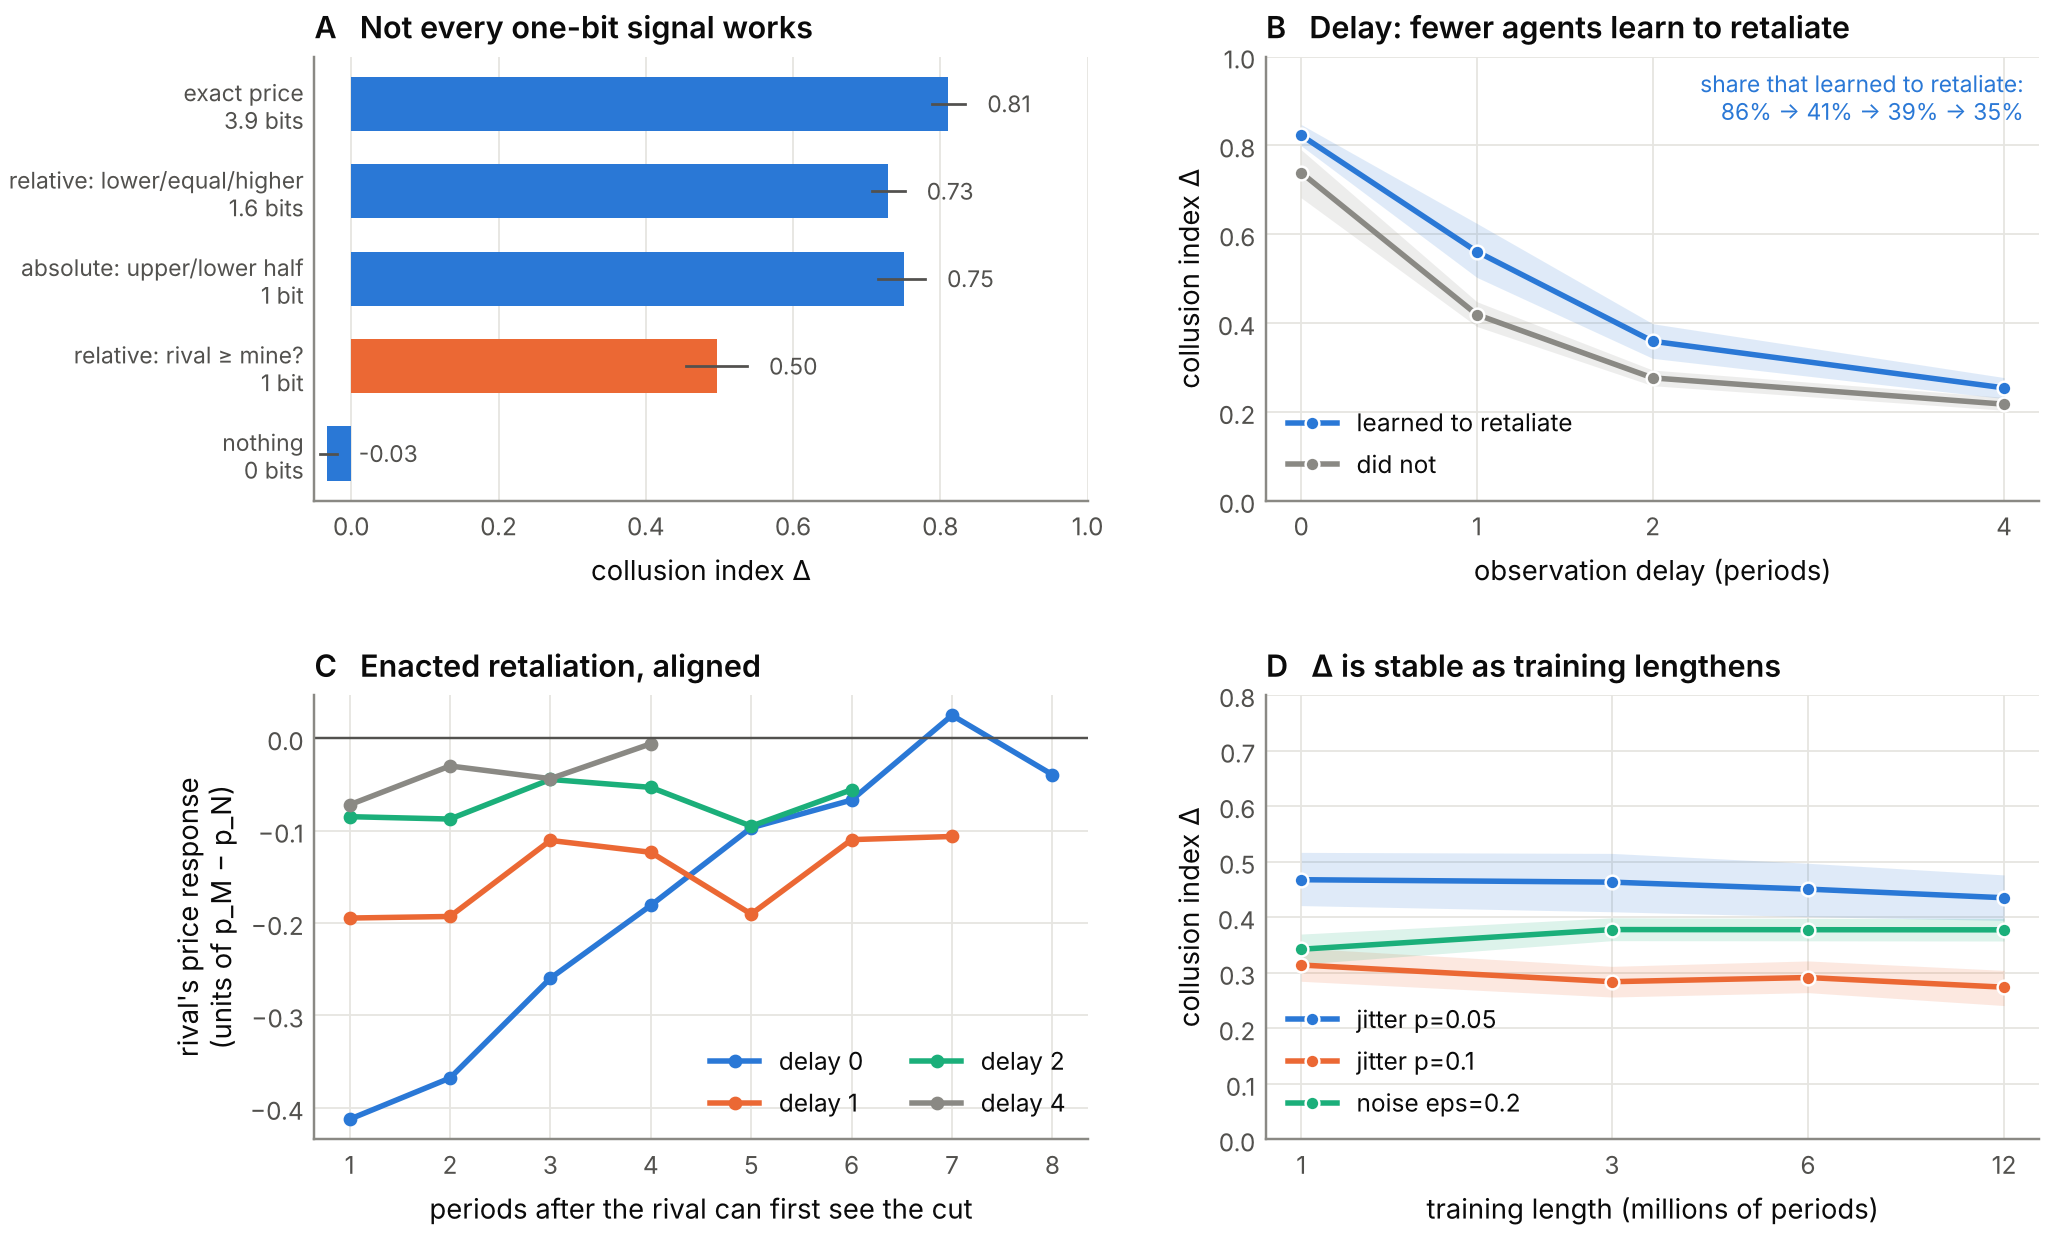
\includegraphics[width=0.82\textwidth,height=\textheight]{figures/mechanisms.png}
\caption{Follow-up experiments (100 sessions per point; 60 in D). (A) Not every one-bit signal sustains collusion. (B) Under delay, fewer agents learn to retaliate, and those that do keep more collusion. (C) The rival's enacted response to a forced cut, aligned to the first period it can see the cut. (D) Δ is stable as training lengthens.}
\end{figure}

\hypertarget{why-does-a-one-period-delay-break-collusion}{%
\subsection{Why does a one-period delay break collusion?}\label{why-does-a-one-period-delay-break-collusion}}

A one-period delay cuts Δ from 0.81 to 0.48, yet a deviation still does not pay (−2.23). Two explanations are natural: punishment arrives too late to deter, or agents fail to learn to retaliate against a delayed signal.

\begin{itemize}
\tightlist
\item
  \textbf{Lateness alone is not enough.} A grim-trigger scheme at γ = 0.95 can sustain the monopoly price even if a deviation goes unpunished for up to 8 periods. A \emph{perfect} trigger strategy would therefore be unaffected by a one-period delay.
\item
  \textbf{Fewer agents learn to retaliate (Figure 3B).} The share of sessions whose learned strategy plans to retaliate falls from 86\% (no delay) to 41\%, 39\% and 35\% (delays of 1, 2 and 4), and mean intended retaliation falls from −0.41 to −0.09. Across sessions, stronger intended retaliation goes with more collusion (correlation −0.52 at one period of delay, −0.48 without delay).
\item
  \textbf{Enacted retaliation is weaker even for agents that learn it (Figure 3C).} With a one-period delay, colluders cut the rival's price by 0.19(\(p_{M}\) − \(p_{N}\)) in the first period they can see the cut, against 0.41 without delay. Sessions that did learn to retaliate reach Δ = 0.56 rather than 0.82.
\end{itemize}

Our reading is that delay mainly makes retaliation harder to \emph{learn}. The agent's state no longer contains the rival's latest price, so the profits it observes depend on information it cannot see, and tabular Q-learning attributes them poorly. Lateness and learning difficulty are confounded in learned agents, so we cannot separate their contributions, and the remaining gap for agents that did learn to retaliate (0.56 against 0.82) is consistent with either. A direct test, giving delayed agents the missing state variable, is future work. The negative deviation gain under delay is not a contradiction: it describes the lower price level these agents settle at, where there is less to gain from deviating.

\hypertarget{does-collusion-survive-swapping-an-agent}{%
\subsection{Does collusion survive swapping an agent?}\label{does-collusion-survive-swapping-an-agent}}

\begin{itemize}
\tightlist
\item
  \textbf{Cross-play.} Pairing agents from different sessions gives Δ = 0.20 (0.17--0.23); only 4\% of pairs exceed 0.5, and punishment vanishes (−0.004). Each pair's prices and triggers are a private convention.
\item
  \textbf{Fresh entrant.} Swapping in a new learner does not break collusion for long: it reaches Δ = 0.74 (0.72--0.76) with an incumbent that keeps learning.
\item
  \textbf{Myopic entrant.} Collusion falls to 0.42.
\item
  \textbf{Frozen incumbent.} A new learner facing an incumbent that no longer learns reaches Δ = 0.62, but a deviation against it now \emph{pays} (+1.54). The entrant has learned to accommodate the incumbent rather than to punish it. This is a high-price outcome with no collusion behind it.
\end{itemize}

\hypertarget{what-evidence-separates-collusion-from-coincidence}{%
\subsection{What evidence separates collusion from coincidence?}\label{what-evidence-separates-collusion-from-coincidence}}

Agents that cannot collude still often price high: 54\% of myopic sessions have Δ \textgreater{} 0.2, and some reach 0.5. Pooled over all controls, price level separates the classes well (AUC 1.00), but only because fully observing colluders price far above everything else. At \textbf{matched price levels} (Figure 2D; 280 pairs, nearly all with a noisy-view colluder, since only those reach the myopic agents' price range):

\begingroup\small
\begin{longtable}[]{@{}ll@{}}
\toprule\noalign{}
Detector & AUC (95\% CI) \\
\midrule\noalign{}
\endhead
\bottomrule\noalign{}
\endlastfoot
D1, price level & 0.48 (0.43--0.53), chance by construction \\
D2, parallel pricing & 0.02 (0.01--0.03): non-colluders move \emph{more} in lockstep \\
D3, lead--lag reaction & 0.91 (0.89--0.93), the best detector \\
D4 / D5, single forced deviation & 0.66 (0.61--0.71) / 0.71 (0.66--0.76) \\
\end{longtable}
\endgroup

Under delay, the immediate punishment signal (D4) reads exactly 0, while D5 still shows that the deviation does not pay. Audits should therefore score the \emph{payoff consequences} of a deviation over a window, not only the immediate reaction.

\hypertarget{what-agents-intend-vs.-what-they-do}{%
\subsection{What agents intend vs.~what they do}\label{what-agents-intend-vs.-what-they-do}}

\begin{figure}
\centering
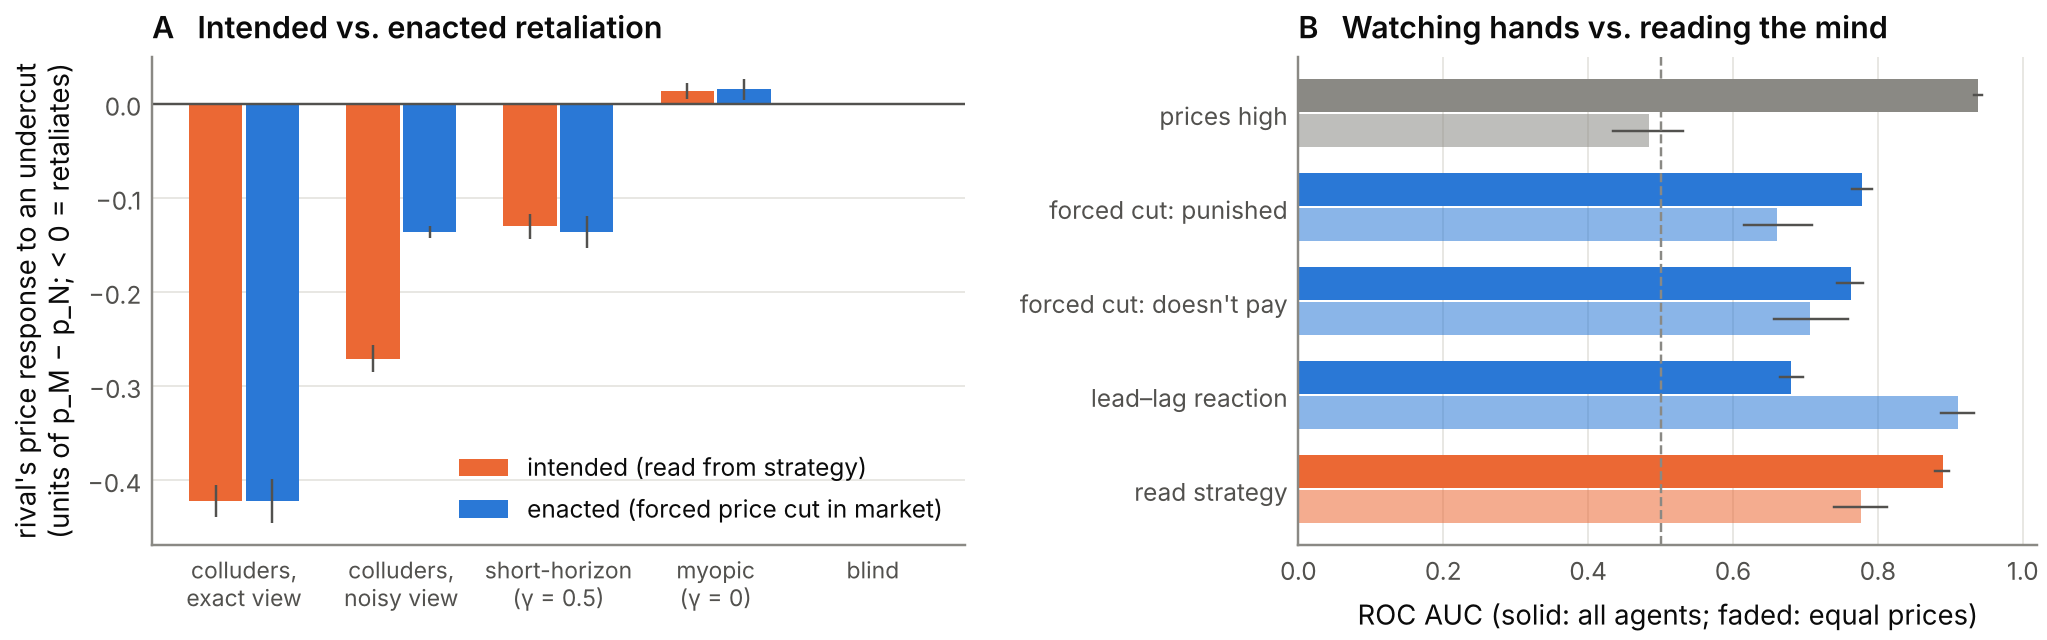
\includegraphics[width=0.95\textwidth,height=\textheight]{figures/mind_vs_hands.png}
\caption{Reading the strategy versus watching behaviour, on the same 5,000 sessions (1,000 per agent type).}
\end{figure}

\begin{itemize}
\tightlist
\item
  \emph{(A)} The rival's retaliation against an undercut: as read from its learned strategy (orange), and as enacted when the undercut is forced in the market (blue). For colluders that see their rival through noise, intended retaliation is about twice the enacted one.
\item
  \emph{(B)} Detection AUC. Solid bars cover all agents; faded bars cover the 280 Δ-matched pairs with equal prices.
\end{itemize}

For colluders with an exact view, reading the strategy and running the market probe agree (−0.42 vs.~−0.42). For colluders who see their rival through noise, they diverge sharply: the strategy plans a cut of −0.27, but in the market the cut is only −0.14. This is because noise also corrupts what the agent perceives \emph{after} the deviation. \textbf{Behaviour understates intent by about half.} Myopic and blind agents plan no retaliation, so reading the strategy never mistakes a coincidental high price for collusion.

As a detector, reading the strategy is the best single test across all agents (AUC 0.89, 0.88--0.90), ahead of the forced-deviation probe (0.76--0.78) and lead--lag reaction (0.68). Raw price level scores 0.94 here, but only because clean colluders price far above everything else, and it falls to chance at equal prices. At equal prices, reading the strategy (0.78, 0.74--0.81) beats a single forced deviation (0.66--0.71). A long passive record of reactions (0.91) remains the strongest test there: it averages over thousands of small natural experiments, whereas we read the strategy at a single state. The two kinds of evidence are complementary. Internals reveal intent that behaviour hides under noise, while long behavioural records reveal how reliably that intent is carried out.

\hypertarget{robustness-and-training-length}{%
\subsection{Robustness and training length}\label{robustness-and-training-length}}

\textbf{Learning parameters.} We repeated the five main levers under Calvano et al.'s slower exploration and under lower and higher learning rates (50 sessions each; Table A4). The ranking never changes. A single absolute bit keeps 87--93\% of baseline collusion, 20\% noise keeps 36--58\%, a one-period delay keeps 49--59\%, and blind agents always price competitively.

\textbf{Does Δ mean anything when sessions do not settle? (Figure 3D; Table A6).} Under noise, non-convergence was a matter of training time: the share of sessions meeting the convergence criterion rises from 2\% at 1 million periods to 98\% at 12 million, while Δ stays at 0.38 (0.36--0.40). Under mandated price jitter, no session can meet a strict criterion by construction, because the forced random prices keep perturbing the learned values. Even so, Δ is stable across a 12-fold longer training run: from 0.47 to 0.44 for p = 0.05 and from 0.31 to 0.27 for p = 0.1, a slight downward drift within the confidence intervals. We therefore read the jitter dose--response as a long-run outcome rather than a fixed point.

\hypertarget{discussion-and-limitations}{%
\section{Discussion and Limitations}\label{discussion-and-limitations}}

\textbf{Implications for AI safety.} As pricing and negotiation are delegated to AI agents, harmful coordination can arise without intent or messages. Our results suggest three rules:

\begin{enumerate}
\def\labelenumi{\arabic{enumi}.}
\tightlist
\item
  \emph{Coordination needs very little bandwidth, but the right bandwidth.} Banding the shared signal to one or two bits is not a safeguard unless the bits fail to separate ``the rival cut'' from ``the rival is at my price''. Randomising or delaying the signal is.
\item
  \emph{Learned conventions are brittle across partners but re-learnable.} Rotating counterparties buys time, not safety.
\item
  \emph{Audits must test reactions, not outcomes.} High and parallel prices are reproduced, and parallelism is even exaggerated, by agents that cannot collude. Because the best passive test needs price variation, a regulator can \emph{induce} that variation, for example with mandated price experiments or sandboxed replays, rather than wait for it.
\end{enumerate}

\textbf{Open questions.} Some of the most important questions remain open:

\begin{itemize}
\tightlist
\item
  \emph{Do LLM agents' notes play the role that Q-tables play here?} That is, does reading what an LLM agent writes reveal intent its prices hide?
\item
  \emph{Faithfulness.} Can an agent's stated reasoning diverge from its actual strategy, and would an auditor notice?
\item
  \emph{Bandwidth.} Does collusion between agents that reason in language need more or fewer bits than Q-learners, and which bits?
\item
  \emph{Concealment.} If agents know they are audited, does intended retaliation migrate into channels that neither prices nor notes reveal?
\end{itemize}

Our LLM extension is built to answer the first three, and its predictions are fixed in advance (Appendix B).

\textbf{Limitations.}

\begin{itemize}
\tightlist
\item
  \emph{Agents.} Our agents are tabular Q-learners with one-period memory, 15 prices and symmetric firms. Agents with longer memory might route around a one-period delay or need more bits.
\item
  \emph{Convergence.} Under jitter no session can meet a strict convergence criterion by construction. Δ is nevertheless stable over a 12-fold longer training run (Section 4.6), so we read the jitter dose--response as a long-run outcome rather than a fixed point.
\item
  \emph{Labels.} ``Collusive'' encodes \emph{capacity} to collude. Short-horizon agents can partly punish, so the headline comparison uses myopic negatives only.
\item
  \emph{Matched sample.} The 280 matched pairs are almost all noisy-view colluders against myopic agents, so the equal-price comparison speaks to that case.
\item
  \emph{Mechanism.} Section 4.2 cannot separate late punishment from difficulty learning it, and our explanation of why delay hinders learning is not tested directly.
\item
  \emph{Welfare.} Welfare effects are specific to this market, where high prices are the only inefficiency. Where price information has legitimate uses, noise and delay carry real costs.
\item
  \emph{No LLM evidence yet.} We did not run the LLM extension during the sprint because we lacked model access. Whether LLM agents share these properties is the main open question. The LLM protocol runs 100 periods per condition before the probe and reports Δ in 20-period blocks, so that a rising trend, rather than a flat low value, flags a horizon that is too short (Appendix B).
\end{itemize}

\textbf{Future work.} The LLM-agent harness (Appendix B) runs the same five conditions, plus a message channel, on Qwen2.5-7B via vLLM. It forks every run at the probe into deviation and no-deviation branches with shared sampling seeds. It also scores agents' private notes with an LLM judge, which lets us compare what agents \emph{say} with what they \emph{do}. The harness is unit-tested with scripted agents, and our predictions are recorded in Appendix B. Further directions: giving delayed agents the missing state variable to test the learning explanation directly, frontier models, longer horizons, asymmetric firms, and steganographic channels.

\textbf{Ethics and dual use.} These results could inform evasion: keeping a coordination signal coarse, or keeping prices deterministic to starve passive audits. We judge the risk low. The properties follow from known trigger-strategy logic, the agents are research-scale, and the main policy implication favours auditors. We release no tooling aimed at real markets.

\hypertarget{conclusion}{%
\section{Conclusion}\label{conclusion}}

Tacit collusion between learning pricing agents travels on the price signal and needs only one or two bits of it, provided those bits let agents recognise a rival's cut. Banding the signal does almost nothing. Random corruption, or a single period of delay, cuts collusion by roughly half, mainly because fewer agents then learn to retaliate, and only removing the signal entirely restores competition. Collusion is a private convention between the agents that learned it: it disappears when partners are swapped and reappears when a new learner enters.

For auditors, high prices and parallel pricing are poor evidence. At equal price levels the first is uninformative and the second points the wrong way. Testing whether firms \emph{react} to rivals' price moves, in a way that makes undercutting unprofitable, separates collusion from coincidence. Looking inside the agents adds a further lesson: behaviour can understate collusive intent by half, so audits with access to an agent's strategy, or to its reasoning, see more than market data alone. Defenders of multi-agent AI systems should target the reliability and timeliness of coordination signals, and auditors should measure reactions rather than outcomes and seek access to internals where possible.

\hypertarget{code-and-data}{%
\section*{Code and Data}\label{code-and-data}}
\addcontentsline{toc}{section}{Code and Data}

\begin{itemize}
\tightlist
\item
  \textbf{Code:} https://github.com/manuaishika/ai-sprint-apart. It contains the market, agents and interventions, the experiment and analysis scripts, unit tests, and the LLM-agent extension (\texttt{collusion\_lab/llm\_market.py}, \texttt{modal\_app.py}).
\item
  \textbf{Data:} session-level results are in \texttt{results/*.csv}, with summaries in \texttt{results/summary.md}.
\item
  \textbf{Reproduce:} \texttt{python\ -m\ experiments.run\_all\ \&\&\ python\ -m\ experiments.robustness\ \&\&\ python\ -m\ experiments.mechanisms\ all\ \&\&\ python\ -m\ experiments.mind\_vs\_hands\ \&\&\ python\ -m\ experiments.analyze\ \&\&\ python\ -m\ experiments.analyze\_mech}. This takes about 90 minutes on 4 CPU cores and needs no GPU or API key.
\end{itemize}

\hypertarget{author-contributions}{%
\section*{Author Contributions}\label{author-contributions}}
\addcontentsline{toc}{section}{Author Contributions}

manuaishika directed the project and chose the research questions. Implementation, experiments and drafting were done with Claude Code (Appendix C).

\hypertarget{references}{%
\section*{References}\label{references}}
\addcontentsline{toc}{section}{References}

\begin{itemize}
\tightlist
\item
  Abada, I., \& Lambin, X. (2023). Artificial intelligence: Can seemingly collusive outcomes be avoided? \emph{Management Science}, 69(9). https://doi.org/10.1287/mnsc.2022.4623
\item
  Asker, J., Fershtman, C., \& Pakes, A. (2022). Artificial intelligence, algorithm design, and pricing. \emph{AEA Papers and Proceedings}, 112. https://doi.org/10.1257/pandp.20221059
\item
  \emph{Audit the Whisper: Detecting Steganographic Collusion in Multi-Agent LLMs} (2025). arXiv:2510.04303. https://arxiv.org/abs/2510.04303
\item
  Calvano, E., Calzolari, G., Denicolò, V., \& Pastorello, S. (2020). Artificial intelligence, algorithmic pricing, and collusion. \emph{American Economic Review}, 110(10), 3267--3297. https://doi.org/10.1257/aer.20190623
\item
  Fish, S., Gonczarowski, Y. A., \& Shorrer, R. I. (2024). Algorithmic collusion by large language models. arXiv:2404.00806. https://arxiv.org/abs/2404.00806
\item
  Garra, A. (2026). Mitigating emergent collusion in LLM pricing agents. arXiv:2609.13037. https://arxiv.org/abs/2609.13037
\item
  Hammond, L., et al.~(2025). Multi-agent risks from advanced AI. arXiv:2502.14143. https://arxiv.org/abs/2502.14143
\item
  Harrington, J. E. (2018). Developing competition law for collusion by autonomous artificial agents. \emph{Journal of Competition Law \& Economics}, 14(3), 331--363. https://doi.org/10.1093/joclec/nhy016
\item
  Johnson, J. P., Rhodes, A., \& Wildenbeest, M. (2023). Platform design when sellers use pricing algorithms. \emph{Econometrica}, 91(5), 1841--1879. https://doi.org/10.3982/ECTA19978
\item
  Klein, T. (2021). Autonomous algorithmic collusion: Q-learning under sequential pricing. \emph{RAND Journal of Economics}, 52(3), 538--558. https://doi.org/10.1111/1756-2171.12383
\item
  Lee, Park (2026). Faithful yet collusive: Why chain-of-thought monitoring cannot detect collusion in LLM pricing agents under oligopolistic competition. arXiv:2609.18346. https://arxiv.org/abs/2609.18346
\item
  Motwani, S. R., et al.~(2024). Secret collusion among AI agents: Multi-agent deception via steganography. arXiv:2402.07510. https://arxiv.org/abs/2402.07510
\end{itemize}

\appendix

\hypertarget{full-results}{%
\section{Full results}\label{full-results}}

\begingroup\small\noindent

\emph{Table A1. All intervention doses (100 sessions each). ``Punish'' is the rival's next-period price response to a forced deviation, in units of \(p_{M}\) − \(p_{N}\). ``Dev. gain'' is the discounted gain from the deviation, in units of \(π_{M}\) − \(π_{N}\); negative means the deviation does not pay.}

\endgroup

\begingroup\small
\begin{longtable}[]{@{}
  >{\raggedright\arraybackslash}p{(\columnwidth - 10\tabcolsep) * \real{0.1667}}
  >{\raggedright\arraybackslash}p{(\columnwidth - 10\tabcolsep) * \real{0.1667}}
  >{\raggedright\arraybackslash}p{(\columnwidth - 10\tabcolsep) * \real{0.1667}}
  >{\raggedright\arraybackslash}p{(\columnwidth - 10\tabcolsep) * \real{0.1667}}
  >{\raggedright\arraybackslash}p{(\columnwidth - 10\tabcolsep) * \real{0.1667}}
  >{\raggedright\arraybackslash}p{(\columnwidth - 10\tabcolsep) * \real{0.1667}}@{}}
\toprule\noalign{}
\begin{minipage}[b]{\linewidth}\raggedright
Intervention
\end{minipage} & \begin{minipage}[b]{\linewidth}\raggedright
Dose
\end{minipage} & \begin{minipage}[b]{\linewidth}\raggedright
Δ
\end{minipage} & \begin{minipage}[b]{\linewidth}\raggedright
Converged
\end{minipage} & \begin{minipage}[b]{\linewidth}\raggedright
Punish
\end{minipage} & \begin{minipage}[b]{\linewidth}\raggedright
Dev. gain
\end{minipage} \\
\midrule\noalign{}
\endhead
\bottomrule\noalign{}
\endlastfoot
baseline & -- & 0.81 & 100\% & −0.41 & −1.34 \\
3 firms & -- & 0.63 & 100\% & −0.28 & −2.98 \\
noise & ε = .05/.1/.2/.4/.7/1 & .68/.58/.38/.18/.01/−.03 & 66/59/50/77/91/94\% & −.32/−.27/−.11/−.04/.00/.00 & −.77/−.55/−.16/−.05/−.01/.00 \\
absolute banding & 8/4/2/1 bands & .82/.74/.75/−.03 & 100\% & −.47/−.34/−.43/.00 & −1.62/−1.56/−1.34/.01 \\
delay & 1/2/4/8 periods & .48/.31/.23/.21 & 100\% & .00 (punishment arrives later) & −2.23/−1.47/−.60/−.35 \\
jitter & p = .02/.05/.1/.2 & .65/.45/.29/.24 & 0\% & −.38/−.22/−.11/−.04 & −1.02/−.50/−.14/.01 \\
\end{longtable}
\endgroup

\begingroup\small\noindent

\emph{Table A2. Agent swaps (100 sessions each).}

\endgroup

\begingroup\small
\begin{longtable}[]{@{}lllll@{}}
\toprule\noalign{}
Condition & Δ (95\% CI) & Share Δ \textgreater{} 0.5 & Punish & Dev. gain \\
\midrule\noalign{}
\endhead
\bottomrule\noalign{}
\endlastfoot
original pair & 0.81 (0.79--0.83) & 99\% & −0.41 & −1.34 \\
cross-play & 0.20 (0.17--0.23) & 4\% & 0.00 & +0.04 \\
fresh learner enters & 0.74 (0.72--0.76) & 97\% & −0.34 & −0.86 \\
fresh learner vs.~frozen incumbent & 0.62 (0.59--0.65) & 77\% & −0.10 & +1.54 \\
myopic entrant & 0.42 (0.38--0.46) & 34\% & −0.18 & −1.39 \\
\end{longtable}
\endgroup

\begingroup\small\noindent

\emph{Table A3. Detection AUC across scenarios. Positives are γ = 0.95 agents; negatives are myopic, short-horizon and blind agents.}

\endgroup

\begingroup\small
\begin{longtable}[]{@{}llllll@{}}
\toprule\noalign{}
Scenario & D1 level & D2 parallel & D3 lead--lag & D4 punish & D5 dev. unprofitable \\
\midrule\noalign{}
\endhead
\bottomrule\noalign{}
\endlastfoot
all agents (4,000 negatives, 1,000 clean-view positives) & 1.00 & 0.73 & 0.64 & 0.81 & 0.86 \\
noisy colluders vs.~all controls (1,000 each) & 0.88 & 0.35 & 0.72 & 0.75 & 0.67 \\
Δ-matched vs.~myopic (280 pairs) & 0.48 & 0.02 & 0.91 & 0.66 & 0.71 \\
\end{longtable}
\endgroup

\begingroup\small\noindent

\emph{Table A4. Mean Δ (95\% CI) under alternative learning parameters (50 sessions per cell). The ranking holds in every setting: one absolute bit leaves most collusion intact, noise and delay roughly halve it, and blindness removes it.}

\endgroup

\begingroup\small
\begin{longtable}[]{@{}
  >{\raggedright\arraybackslash}p{(\columnwidth - 10\tabcolsep) * \real{0.1667}}
  >{\raggedright\arraybackslash}p{(\columnwidth - 10\tabcolsep) * \real{0.1667}}
  >{\raggedright\arraybackslash}p{(\columnwidth - 10\tabcolsep) * \real{0.1667}}
  >{\raggedright\arraybackslash}p{(\columnwidth - 10\tabcolsep) * \real{0.1667}}
  >{\raggedright\arraybackslash}p{(\columnwidth - 10\tabcolsep) * \real{0.1667}}
  >{\raggedright\arraybackslash}p{(\columnwidth - 10\tabcolsep) * \real{0.1667}}@{}}
\toprule\noalign{}
\begin{minipage}[b]{\linewidth}\raggedright
Setting
\end{minipage} & \begin{minipage}[b]{\linewidth}\raggedright
None
\end{minipage} & \begin{minipage}[b]{\linewidth}\raggedright
1 absolute bit
\end{minipage} & \begin{minipage}[b]{\linewidth}\raggedright
20\% noise
\end{minipage} & \begin{minipage}[b]{\linewidth}\raggedright
1-period delay
\end{minipage} & \begin{minipage}[b]{\linewidth}\raggedright
Blind
\end{minipage} \\
\midrule\noalign{}
\endhead
\bottomrule\noalign{}
\endlastfoot
main (α = 0.15, β = \(10^{-5}\); 100 sessions) & 0.81 (0.79--0.83) & 0.75 (0.71--0.78) & 0.38 (0.37--0.40) & 0.48 (0.45--0.51) & −0.03 \\
slower exploration (β = 4×\(10^{-6}\), as in Calvano et al.) & 0.83 (0.79--0.86) & 0.76 (0.71--0.80) & 0.30 (0.28--0.32) & 0.41 (0.37--0.46) & −0.03 \\
lower learning rate (α = 0.1) & 0.81 (0.78--0.84) & 0.74 (0.69--0.78) & 0.47 (0.45--0.49) & 0.48 (0.44--0.52) & −0.05 \\
higher learning rate (α = 0.25) & 0.83 (0.79--0.86) & 0.72 (0.66--0.77) & 0.34 (0.32--0.36) & 0.42 (0.38--0.47) & −0.04 \\
\end{longtable}
\endgroup

\begingroup\small\noindent

\emph{Table A5. Delay mechanism (100 sessions per delay). ``Learned'' is the share of sessions whose strategy plans to retaliate (intended retaliation below −0.1 in units of \(p_{M}\) − \(p_{N}\)); ``intended'' is its mean.}

\endgroup

\begingroup\small
\begin{longtable}[]{@{}lllll@{}}
\toprule\noalign{}
Delay (periods) & Δ & Learned & Intended & Corr(Δ, intended) \\
\midrule\noalign{}
\endhead
\bottomrule\noalign{}
\endlastfoot
0 & 0.81 & 86\% & −0.41 & −0.48 \\
1 & 0.48 & 41\% & −0.09 & −0.52 \\
2 & 0.31 & 39\% & −0.07 & −0.39 \\
4 & 0.23 & 35\% & −0.06 & −0.25 \\
\end{longtable}
\endgroup

\begingroup\small\noindent

\emph{Table A6. Δ by training length (60 sessions per cell; 95\% CI). ``Converged'' is the share of sessions meeting the strict convergence criterion.}

\endgroup

\begingroup\small
\begin{longtable}[]{@{}lllll@{}}
\toprule\noalign{}
Condition & 1M periods & 3M & 6M & 12M \\
\midrule\noalign{}
\endhead
\bottomrule\noalign{}
\endlastfoot
jitter p = 0.05 & 0.47 (0.42--0.52) & 0.46 (0.41--0.51) & 0.45 (0.40--0.50) & 0.44 (0.39--0.48) \\
jitter p = 0.1 & 0.31 (0.28--0.34) & 0.28 (0.26--0.31) & 0.29 (0.26--0.32) & 0.27 (0.24--0.30) \\
noise ε = 0.2 & 0.34 (0.32--0.37) & 0.38 (0.36--0.40) & 0.38 (0.36--0.40) & 0.38 (0.36--0.40) \\
noise ε = 0.2, converged & 2\% & 43\% & 93\% & 98\% \\
\end{longtable}
\endgroup

\hypertarget{llm-agent-extension-protocol-and-pre-registered-predictions}{%
\section{LLM-agent extension: protocol and pre-registered predictions}\label{llm-agent-extension-protocol-and-pre-registered-predictions}}

\texttt{collusion\_lab/llm\_market.py} places LLM pricing agents in the same market, following Fish et al.~(2024). \texttt{modal\_app.py} runs them with Qwen2.5-7B-Instruct via vLLM.

\textbf{Prompts.} Each period, an agent receives:

\begin{itemize}
\tightlist
\item
  its marginal cost and the goal ``maximise long-run profit'';
\item
  the last 20 periods of its own price, sales and profit;
\item
  the condition's view of the competitor's price;
\item
  its notes from the previous period.
\end{itemize}

It replies in JSON with new notes and a price.

\textbf{Conditions.} Six conditions, each with 10 seeds and 100 periods before the probe (plus 10 after):

\begin{itemize}
\tightlist
\item
  exact price;
\item
  relative: lower / about the same / higher than the agent's own price (the Q-learning analogue is the three-valued relative signal, Δ = 0.73);
\item
  30\% noise;
\item
  one period late;
\item
  blind;
\item
  exact price plus a free-text message channel.
\end{itemize}

\textbf{Probe.} At period 100, every run forks into a branch where firm 0 is forced to its one-shot best response and a branch where it is not. The two branches share sampling seeds.

\textbf{Detectors.} The five behavioural detectors above, plus two text-based ones: a coordination-word lexicon applied to agents' notes, and an LLM judge that rates the notes from 0 to 10.

The pipeline is unit-tested with scripted agents. We have not yet run it with a real model. Predictions, recorded before any LLM run:

\begin{itemize}
\tightlist
\item
  \textbf{P1.} With the exact price, Δ \textgreater{} 0.3.
\item
  \textbf{P2.} The conditions keep the RL ordering: exact ≥ relative \textgreater{} delayed, noisy \textgreater{} blind.
\item
  \textbf{P3.} Blind LLM agents still price above Nash (Δ \textgreater{} 0.1).
\item
  \textbf{P4.} Price level and parallel pricing fail to separate exact-price agents from blind ones, while reaction and probe tests succeed.
\item
  \textbf{P5.} The judge of private notes separates them at least as well as behaviour.
\item
  \textbf{P6.} The message channel raises collusion.
\item
  \textbf{P7.} The horizon is long enough: in the exact-price condition, mean Δ in the last two 20-period blocks before the probe differs by less than 0.1.
\end{itemize}

\textbf{Horizon.} Q-learners train for up to millions of periods, whereas LLM agents adapt in context and condition on a 20-period window, so 100 periods give them several full windows. The analysis reports Δ per 20-period block (\texttt{results/llm\_summary.md}). A flat low value in the exact-price condition together with a flat blind control is evidence of no collusion; a clear upward slope in the last blocks would mean the horizon was too short, and we would extend it before concluding anything.

\hypertarget{llm-usage-statement}{%
\section{LLM usage statement}\label{llm-usage-statement}}

We used Claude (via Claude Code) extensively:

\begin{itemize}
\tightlist
\item
  to implement the simulation, experiment and analysis code;
\item
  to run the experiments;
\item
  to produce the figures;
\item
  to draft this report.
\end{itemize}

All reported numbers are generated by code in the repository from logged results, and the code is covered by unit tests. The research questions and final editorial decisions are the author's.

\end{document}
